\documentclass[11pt,a4paper]{article}

\usepackage[T2A]{fontenc}
\usepackage[utf8]{inputenc}
\usepackage[english,russian]{babel}

\usepackage[a4paper, 
            lmargin=0.1666\paperwidth, 
            rmargin=0.1666\paperwidth, 
            tmargin=0.1111\paperheight, 
            bmargin=0.1111\paperheight]{geometry}

\usepackage{mathptmx}
\usepackage{amsmath}
\usepackage{amssymb}

\usepackage{graphicx}
\usepackage{float}

\usepackage{array}
\usepackage{enumitem}
\usepackage{hyperref}

\title{Стохастические методы обучения}
\author{Евгений Баяк}
\date{Март 2025}

\begin{document}

\maketitle

\section*{Введение}
Современный мир характеризуется активным переходом к цифровизации, в связи с чем машинное обучение приобретает ключевое значение в различных областях науки и техники. Одним из наиболее перспективных направлений в данной сфере являются стохастические методы обучения, основанные на применении случайных процессов и вероятностных моделей для оптимизации процессов обучения.

Актуальность данных методов обусловлена высокой степенью неопределенности и изменчивости данных, с которыми сталкиваются современные системы. Стохастические подходы позволяют не только повысить точность моделей, но и существенно сократить время их обучения. Важно подчеркнуть, что применение стохастических методов широко распространено в таких областях, как финансовый анализ, обработка естественного языка, компьютерное зрение и других.

Исследование стохастических методов обучения представляет собой значимую научную задачу, решение которой способствует дальнейшему развитию технологий и повышению их эффективности в практических приложениях.


\section{Основные понятия стохастических методов обучения}

\subsection{Понятие стохастичности в обучении}
Стохастические методы обучения представляют собой важный раздел машинного обучения, который использует случайность как инструмент для оптимизации процессов обучения моделей. Эти методы особенно эффективны в задачах с большими объемами данных, где детерминированные подходы могут быть вычислительно затратными или неэффективными. Основная идея заключается в том, чтобы вместо обработки всего набора данных целиком использовать случайные подмножества (выборки) для итеративного улучшения параметров модели. Такой подход позволяет сократить время вычислений и адаптироваться к изменяющимся условиям задачи.

Стохастичность в контексте машинного обучения означает введение элемента случайности в процесс обучения модели. Это может проявляться в выборе случайных подвыборок данных (mini-batches) для каждой итерации оптимизации, случайной инициализации параметров модели или добавлении шума в вычисления для повышения обобщающей способности. В отличие от детерминированных методов, где результат полностью предсказуем при заданных входных данных, стохастические методы генерируют решения, которые могут варьироваться от запуска к запуску.

Примером стохастичности является алгоритм стохастического градиентного спуска. В традиционном градиентном спуске для вычисления градиента функции потерь используется весь набор данных, что требует значительных вычислительных ресурсов. В стохастической версии градиент оценивается на основе одного случайно выбранного примера или небольшой группы примеров. Это ускоряет процесс обучения, особенно на больших датасетах, но приводит к шумным обновлениям параметров, что требует дополнительных техник, таких как уменьшение шага обучения (learning rate decay), для достижения сходимости.

Стохастичность выступает как компромисс между точностью и вычислительной эффективностью, позволяя решать задачи машинного обучения в условиях ограниченных ресурсов и неопределенности.


\subsection{Различие между детерминированными и стохастическими подходами}
Детерминированные и стохастические подходы представляют два фундаментально разных способа моделирования и обучения, отличающихся по степени использования случайности и эффективности на различных типах данных. 

Детерминированные методы -- это алгоритмы, при которых результат полностью определяется входными данными и параметрами модели, без какого-либо элемента случайности. Это означает, что для одних и тех же входных данных модель всегда будет давать один и тот же выход, что делает их предсказуемыми и воспроизводимыми. Например, полный градиентный спуск использует весь набор данных для вычисления градиента и обновления параметров, что исключает случайность.

Стохастические методы, напротив, включают элемент случайности, что делает результаты непредсказуемыми даже при одинаковых входных данных. Это достигается, например, за счет использования случайных подвыборок данных или случайной инициализации параметров. Стохастический градиентный спуск (SGD) -- классический пример, где модель обновляется на основе мини-пакетов данных, выбранных случайным образом. Основное различие заключается в том, что детерминированные методы исключают неопределенность, в то время как стохастические методы используют её для повышения эффективности и гибкости. В таблице \ref{table:1} описаны преимущества и недостатки детерминированного и стохастического методов~\cite{askpython}.

\begin{table}
	\caption{Анализ детерминированного и стохастического методов}
	\label{table:1}
	\begin{tabular}{|p{0.12\textwidth}|>{\raggedright\arraybackslash}p{0.39\textwidth}|>{\raggedright\arraybackslash}p{0.39\textwidth}|}
		\hline
		Аспект & Детерминированные методы & Стохастические методы \\
		\hline
		Преиму\-щества  & \begin{itemize}[leftmargin=*,label=--, nosep] 
		\item Предсказуемые и воспроизводимые результаты;
		\item Легче интерпретировать и отлаживать.
		\end{itemize}
		        
		& \begin{itemize}[leftmargin=*,label=--, nosep]
		\item Быстрее обучаются на больших наборах данных;
		\item Могут избегать локальных минимумов;
		\item Улучшают обобщающую способность.
		\end{itemize} \\
		\hline
		Недо\-статки & \begin{itemize}[leftmargin=*,label=--, nosep]
		\item Вычислительно затратны для больших данных;
		\item Могут застревать в локальных минимумах.
		\end{itemize}
		& \begin{itemize}[leftmargin=*,label=--, nosep]
		\item Результаты варьируются между запусками;
		\item Труднее интерпретировать;
		\item Требуют настройки гиперпараметров.
		\end{itemize} \\
		\hline
	\end{tabular}
\end{table}


\subsection{Преодоление локального минимума}

Одним из ключевых преимуществ стохастических методов является способность помогать модели избегать локальных минимумов в процессе оптимизации. Рисунок \ref{fig:fig1} иллюстрирует этот процесс.

\begin{figure}[H]
    \centering
    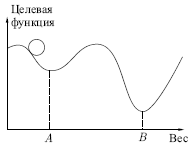
\includegraphics[width=0.5\linewidth]{local-minimum-ball.png}
    \caption{Минимизация целевой функции}
    \label{fig:fig1}
\end{figure}

Детерминированный и стохастический подходы рассмотрены на примере градиентного спуска. На рисунке мяч начинает движение с некоторой начальной точки на поверхности, представляющей значения функции потерь в зависимости от параметров модели. В детерминированном подходе мяч будет катиться строго вниз по наиболее крутому склону, пока не остановится в ближайшей впадине -- локальном минимуме \(A\). Это происходит потому, что обновления параметров в таких методах основаны на точном вычислении градиента по всему набору данных, что приводит к предсказуемому движению к ближайшей точке минимума. Однако локальный минимум \(A\) может быть значительно хуже глобального минимума \(B\) с точки зрения общей ошибки модели, что делает такой результат нежелательным.

В отличие от детерминированного подхода, случайное обновление параметров вводит элемент шума в процесс движения мячика. Вместо того чтобы строго следовать градиенту всего набора данных, параметры обновляются на основе случайных мини-пакетов, что эквивалентно небольшим случайным толчкам мячика в разные стороны. Этот шум может выбить мяч из локального минимума \(A\), позволяя ему продолжить движение и, в конечном итоге, достичь глобального минимума \(B\). На изображении это можно представить как ситуацию, где мячик, застрявший в точке \(A\), получает случайный импульс, который выводит его из впадины и направляет к более глубокой точке \(B\)~\cite{intuit}.


\section{Стохастический градиентный спуск}

Стохастический градиентный спуск является одним из наиболее популярных и широко используемых методов оптимизации в машинном обучении. Этот метод представляет собой стохастическую версию классического градиентного спуска, где параметры модели обновляются на основе случайных подмножеств данных (мини-пакетов) вместо полного набора данных. Благодаря своей вычислительной эффективности и способности работать с большими объемами данных, SGD стал основой для обучения сложных моделей, таких как нейронные сети. В данном разделе мы рассмотрим математическую основу SGD, алгоритм его работы и примеры применения в задачах машинного обучения.

SGD особенно ценен в ситуациях, когда обработка всего набора данных на каждой итерации становится вычислительно невозможной или неэффективной. Введение случайности позволяет не только ускорить процесс обучения, но и улучшить обобщающую способность модели за счет эффекта регуляризации, который возникает из-за шума в обновлениях параметров. Однако это также делает метод чувствительным к настройке гиперпараметров, таких как скорость обучения, и требует дополнительных техник для обеспечения стабильной сходимости.

\subsection{Математическая основа SGD}
Математическая основа стохастического градиентного спуска базируется на идее минимизации функции потерь, которая измеряет ошибку модели на обучающих данных. Пусть дана обучающая выборка 
\begin{equation}
\{(x_i, y_i)\}_{i=1}^N
\end{equation}
где \( x_i \) — входные данные, \( y_i \) — целевые значения, а \( N \) — общее число примеров. Целью является нахождение оптимальных параметров модели \( \theta \), которые минимизируют функцию потерь \( J(\theta) \), определенную как:
\begin{equation}
J(\theta) = \frac{1}{N} \sum_{i=1}^N L(\theta; x_i, y_i)
\end{equation}
где \( L(\theta; x_i, y_i) \) — функция потерь для отдельного примера, зависящая от параметров \( \theta \). Например, в задаче регрессии это может быть среднеквадратичная ошибка, а в задаче классификации — кросс-энтропия.

В традиционном градиентном спуске обновление параметров выполняется путем вычисления градиента функции потерь по всему набору данных:
\begin{equation}
\theta = \theta - \eta \nabla_\theta J(\theta) = \theta - \eta \frac{1}{N} \sum_{i=1}^N \nabla_\theta L(\theta; x_i, y_i)
\end{equation}
где \( \eta \) — скорость обучения (learning rate), а \( \nabla_\theta J(\theta) \) — градиент функции потерь. Однако для больших \( N \) это вычисление становится слишком затратным.

В отличие от этого, SGD использует приближенную оценку градиента, вычисляемую по одному случайно выбранному примеру или мини-пакету. Для одного примера обновление параметров записывается как:
\begin{equation}
\theta = \theta - \eta \nabla_\theta L(\theta; x_i, y_i)
\end{equation}
где индекс \( i \) выбирается случайным образом из множества \( \{1, 2, \dots, N\} \). Для мини-пакета размером \( B \) обновление принимает вид:
\begin{equation}
\theta = \theta - \eta \frac{1}{B} \sum_{i \in B} \nabla_\theta L(\theta; x_i, y_i)
\end{equation}
где \( B \) — случайное подмножество примеров из обучающей выборки. Случайный выбор примеров или мини-пакетов делает процесс стохастическим, что отличает SGD от детерминированного градиентного спуска.

Этот подход основан на предположении, что градиент по одному примеру или мини-пакету является шумной, но в среднем непредвзятой оценкой истинного градиента по всему набору данных. Математически это выражается через ожидание:
\begin{equation}
\mathbb{E}[\nabla_\theta L(\theta; x_i, y_i)] = \nabla_\theta J(\theta)
\end{equation}
где ожидание берется по случайному выбору примеров. Таким образом, многократные итерации SGD позволяют приблизиться к оптимальным параметрам \( \theta^* \), минимизирующим \( J(\theta) \).

\subsection{Алгоритм работы SGD}

Алгоритм стохастического градиентного спуска представляет собой итеративный процесс, который можно описать пошагово. Он прост в реализации, но требует внимания к выбору скорости обучения и размера мини-пакета. 

Алгоритм заключается в следующем.

Параметры $\theta$ инициализируются случайным образом. Задаются скорость обучения $\eta$, размер мини-пакета $B$ и максимальное число эпох $T$.

Для каждой эпохи $t = 1, 2, \dots, T$: 
\begin{enumerate}
    \item Обучающая выборка $\{(x_i, y_i)\}_{i=1}^N$ перемешивается для обеспечения случайного порядка примеров.
    \item Данные разбиваются на мини-пакеты размером $B$.
    \item Для каждого мини-пакета $b$ вычисляется градиент функции потерь:
    \begin{equation}
    g_b = \frac{1}{B} \sum_{i \in b} \nabla_\theta L(\theta; x_i, y_i)
    \end{equation}
    Затем параметры обновляются по формуле:
   \begin{equation}
    \theta = \theta - \eta g_b
    \end{equation}
\end{enumerate}

На каждой эпохе можно оценить значение функции потерь на валидационной выборке. Обучение прекращается, если достигнута приемлемая точность или изменения параметров $\theta$ становятся незначительными.

Алгоритм возвращает оптимизированные параметры $\theta$.

Этот алгоритм отличается от полного градиентного спуска тем, что обновления происходят чаще (на каждом мини-пакете), а не после обработки всего набора данных. Перемешивание данных перед каждой эпохой гарантирует, что модель не запоминает порядок примеров, что улучшает обобщение. Размер мини-пакета \( B \) является компромиссом: 
\begin{equation}
B = 1
\end{equation}
соответствует чистому SGD с максимальным шумом, а большие \( B \) (например, 32 или 64) уменьшают шум, приближая метод к пакетному градиентному спуску.

\subsection{Примеры использования в задачах машинного обучения}
Стохастический градиентный спуск широко применяется в машинном обучении благодаря своей универсальности и эффективности. Он особенно полезен в задачах с большими объёмами данных, где полный градиентный спуск вычислительно неэффективен.

В задачах предсказания непрерывных значений SGD минимизирует среднеквадратичную ошибку. При работе с миллионами записей о недвижимости SGD обновляет коэффициенты модели, обрабатывая данные по мини-пакетам. Это позволяет ускорить обучение и адаптироваться к потоковой обработке данных.

Для задач бинарной классификации SGD минимизирует функцию потерь кросс-энтропии. Он эффективен при работе с большими текстовыми датасетами, где обработка всех данных за один раз невозможна. Например, SGD обновляет веса модели на основе случайных подмножеств писем, что значительно ускоряет обучение.

В задачах распознавания изображений SGD оптимизирует параметры глубоких нейронных сетей с миллионами весов. В сверточных нейронных сетях мини-пакеты размером 32--256 позволяют обучать модели на огромных датасетах. Для ускорения сходимости часто используются модификации, такие как Adam или RMSprop.

В задачах оптимизации политики агента SGD обновляет параметры нейронной сети, представляющей Q-функцию или политику. В алгоритмах Deep Q-Learning SGD работает с выборками из буфера опыта (experience replay), что делает обучение устойчивым к корреляциям в последовательных данных.

Эти примеры показывают, что SGD универсален и адаптируется к различным задачам. Его способность работать с большими данными и избегать локальных минимумов делает его ключевым инструментом в современных приложениях машинного обучения.


\section{Улучшенные версии SGD}

Хотя стохастический градиентный спуск является эффективным методом оптимизации для задач машинного обучения, его базовая версия имеет ряд ограничений. К ним относятся нестабильность обновлений параметров из-за высокого уровня шума и чувствительность к выбору скорости обучения. Для устранения этих недостатков были разработаны улучшенные версии SGD, которые повышают стабильность, ускоряют сходимость и адаптируются к различным типам данных и задач.

Эти улучшенные версии сохраняют стохастическую природу базового метода, но добавляют механизмы, повышающие устойчивость процесса обучения. Их использование стало стандартом в машинном обучении благодаря сочетанию вычислительной эффективности и способности адаптироваться к сложным ландшафтам функций потерь.

\subsection{Mini-batch SGD}

Mini-batch SGD (мини-пакетный стохастический градиентный спуск) представляет собой компромисс между классическим SGD, где используется один пример на итерацию, и полным градиентным спуском, где обрабатывается весь набор данных. В этом подходе параметры модели обновляются на основе небольшого подмножества данных, называемого мини-пакетом, размер которого обычно варьируется от 32 до 256 примеров.

В Mini-batch SGD обучающая выборка 
\begin{equation}
\{(x_i, y_i)\}_{i=1}^N
\end{equation}
делится на мини-пакеты размером \( B \). На каждой итерации выбирается случайный мини-пакет \( b \), и градиент функции потерь вычисляется как среднее по этому подмножеству:
\begin{equation}
g_b = \frac{1}{B} \sum_{i \in b} \nabla_\theta L(\theta; x_i, y_i)
\end{equation}
где \( \theta \) — параметры модели, \( \eta \) — скорость обучения, а обновление параметров записывается как:
\begin{equation}
\theta = \theta - \eta g_b
\end{equation}
Перед каждой эпохой данные перемешиваются, чтобы обеспечить случайный порядок мини-пакетов, что улучшает обобщающую способность модели.

Mini-batch SGD снижает уровень шума по сравнению с чистым SGD, где на каждой итерации используется только один пример. Применение мини-пакетов уменьшает вариативность градиента, что делает обновления параметров более стабильными. Кроме того, размер мини-пакета позволяет эффективно использовать современные вычислительные архитектуры, например, GPU, где параллельные вычисления ускоряют обработку нескольких примеров одновременно. Mini-batch SGD сохраняет способность избегать локальных минимумов, при этом приближаясь к точности полного градиентного спуска с увеличением размера мини-пакета.

Одним из недостатков Mini-batch SGD является необходимость выбора размера мини-пакета, который требует баланса. Слишком маленький размер сохраняет высокий уровень шума, а слишком большой приближает метод к пакетному градиентному спуску, что может снизить вычислительную эффективность. Кроме того, Mini-batch SGD, как и базовый SGD, чувствителен к скорости обучения, что может потребовать использования дополнительных техник, например, затухания скорости обучения.

Mini-batch SGD стал де-факто стандартом в обучении глубоких нейронных сетей, где большие объемы данных и вычислительные ограничения делают полный градиентный спуск непрактичным, а чистый SGD — слишком нестабильным.

\subsection{RMSProp, Adam и их модификации}

Адаптивные методы оптимизации представляют собой следующую ступень эволюции SGD, устраняя его зависимость от фиксированной скорости обучения и улучшая сходимость за счёт динамической адаптации к градиентам.

RMSProp (Root Mean Square Propagation) был предложен для адаптации скорости обучения для каждого параметра на основе экспоненциально затухающего среднего квадратов прошлых градиентов. Алгоритм работает следующим образом:

Вычисляется экспоненциальное среднее квадрата градиента:
\begin{equation}
E[g^2]_t = \rho E[g^2]_{t-1} + (1 - \rho) g_t^2
\end{equation}
где \( g_t = \nabla_\theta L(\theta; x_t, y_t) \), \( \rho \) — коэффициент затухания (обычно 0.9).

Обновление параметров:
\begin{equation}
\theta = \theta - \frac{\eta}{\sqrt{E[g^2]_t + \epsilon}} g_t
\end{equation}
где \( \epsilon \) — малая константа (например, \( 10^{-8} \)) для предотвращения деления на ноль.

RMSProp уменьшает скорость обучения для параметров с большими градиентами и увеличивает её для параметров с малыми градиентами, что ускоряет сходимость в задачах с неоднородными масштабами параметров.

Adam (Adaptive Moment Estimation) сочетает идеи RMSProp и метода моментума, используя как первое (средний градиент), так и второе (средний квадрат градиента) моменты. Алгоритм включает:

Вычисление экспоненциального среднего градиента (моментум):
\begin{equation}
m_t = \beta_1 m_{t-1} + (1 - \beta_1) g_t
\end{equation}
где \( \beta_1 \) — коэффициент затухания (обычно 0.9).

Вычисление экспоненциального среднего квадрата градиента:
\begin{equation}
v_t = \beta_2 v_{t-1} + (1 - \beta_2) g_t^2
\end{equation}
где \( \beta_2 \) — коэффициент затухания (обычно 0.999).

Коррекция смещения для начальных итераций:
\begin{equation}
\hat{m}_t = \frac{m_t}{1 - \beta_1^t}, \quad \hat{v}_t = \frac{v_t}{1 - \beta_2^t}
\end{equation}

Обновление параметров:
\begin{equation}
\theta = \theta - \frac{\eta}{\sqrt{\hat{v}_t} + \epsilon} \hat{m}_t
\end{equation}

Adam адаптирует скорость обучения для каждого параметра, учитывая как направление (через \( m_t \)), так и масштаб (через \( v_t \)) градиента. Это делает его эффективным для сложных функций потерь.

Модификации:
\begin{itemize}[label=--]
    \item Nadam;
    \item AMSGrad.
\end{itemize}

Nadam добавляет метод Нестерова к Adam, улучшая учет инерции градиента. AMSGrad исправляет проблему Adam с возможным увеличением скорости обучения на поздних стадиях, заменяя \( \hat{v}_t \) на максимум прошлых значений \( v_t \). Эти методы широко применяются в задачах глубокого обучения, где требуется быстрая сходимость и устойчивость к шуму.

\subsection{Сравнение методов}

Для выбора подходящего метода оптимизации важно понимать их различия в эффективности, скорости сходимости и применимости. В таблице \ref{table:2} сравнены Mini-batch SGD, RMSProp и Adam на основе ключевых характеристик.

\begin{table}
    \caption{Сравнение методов оптимизации}
    \setlength{\tabcolsep}{3pt}
    \label{table:2}
    \begin{tabular}{|>{\raggedright\arraybackslash}p{0.2\textwidth}|>{\raggedright\arraybackslash}p{0.24\textwidth}|>{\raggedright\arraybackslash}p{0.24\textwidth}|>{\raggedright\arraybackslash}p{0.24\textwidth}|}
    \hline
    \textbf{Характеристи\-ка} & \textbf{Mini-batch SGD} & \textbf{RMSProp} & \textbf{Adam} \\ \hline
    Скорость обучения & Фиксированная, требует ручной настройки & Адаптивная для каждого параметра & Адаптивная с учетом моментума \\ \hline
    Сходимость & Медленная, шумная & Быстрее, чем SGD, но может колебаться & Быстрая и стабильная \\ \hline
    Вычислитель\-ная сложность & Низкая & Средняя (дополнительные средние) & Высокая (два момента + коррекция) \\ \hline
    Устойчивость к шуму & Умеренная (зависит от \( B \)) & Высокая & Очень высокая \\ \hline
    Применимость & Простые модели, большие данные & Нейронные сети, неоднородные данные & Глубокие сети, сложные задачи \\ \hline
    \end{tabular}
\end{table}

Mini-batch SGD демонстрирует высокую эффективность при работе с большими объемами данных, поскольку требует минимального объема памяти. Однако сходимость данного метода может быть замедленной, особенно в случае плохо обусловленных функций потерь. В отличие от Mini-batch SGD, алгоритм RMSProp ускоряет сходимость за счет адаптивной настройки скорости обучения, что делает его более подходящим для задач с разреженными или неоднородными данными.

Алгоритм Adam, в свою очередь, обеспечивает быструю и стабильную сходимость, что делает его предпочтительным выбором для обучения глубоких нейронных сетей, включая сверточные и рекуррентные сети. Это особенно важно в задачах с большим количеством параметров и сложным ландшафтом функций потерь.

Mini-batch SGD прост в реализации, но требует тщательной настройки \( \eta \) и размера мини-пакета. Он может застревать в локальных минимумах без дополнительных техник, например, моментума. RMSProp устойчив к резким изменениям градиентов, но может быть нестабильным на поздних стадиях обучения из-за накопления шума в \( E[g^2] \). Adam сочетает преимущества моментума и RMSProp, но более требователен к вычислительным ресурсам. Иногда он демонстрирует худшую обобщающую способность на тестовых данных по сравнению с SGD с моментумом, что привело к разработке AMSGrad.

Mini-batch SGD с моментумом достаточно для простых задач с небольшими данными. Для задач с разреженными данными RMSProp часто предпочтительнее. Для глубокого обучения, например, в компьютерном зрении, Adam обычно является выбором по умолчанию благодаря скорости и устойчивости, хотя иногда его заменяют SGD с затуханием \( \eta \) для лучшего обобщения \cite{goodfellow}.


\section*{Заключение}

Стохастические методы обучения занимают центральное место в современном машинном обучении, обеспечивая эффективные инструменты для оптимизации моделей в условиях больших объёмов данных и сложных функций потерь.

Стохастичность в обучении, несмотря на введение шума и нестабильности, предоставляет значительные преимущества по сравнению с детерминированными подходами, включая вычислительную эффективность и способность избегать локальных минимумов. SGD, как основной представитель стохастических методов, демонстрирует универсальность благодаря своей математической простоте и применимости к широкому спектру задач — от линейной регрессии до глубоких нейронных сетей. Его алгоритм, основанный на случайных обновлениях параметров, позволяет масштабировать обучение на большие датасеты, что делает его незаменимым в современных приложениях.

SGD Mini-batch SGD, RMSProp и Adam и другие улучшенные версии устраняют многие недостатки базового метода, повышая стабильность и скорость сходимости. Mini-batch SGD балансирует между шумом и точностью, адаптивные методы динамически корректируют процесс обучения, что особенно важно для сложных моделей глубокого обучения. Стохастические методы продолжают оставаться основой для достижения высоких результатов в области машинного обучения, обеспечивая гибкость и эффективность в решении разнообразных задач.


\begin{thebibliography}{9}
\bibitem{askpython}
AskPython: Deterministic vs Stochastic -- Machine Learning (Fundamentals) [Электронный ресурс]. -- Режим доступа: \url{https://www.askpython.com/python/examples/deterministic-vs-stochastic-machine-learning}. -- Дата доступа: 23.03.2025.

\bibitem{intuit}
НОУ ИНТУИТ | Основы теории нейронных сетей. Лекция 7: Стохастические методы обучения нейронных сетей [Электронный ресурс]. -- Режим доступа: \url{https://intuit.ru/studies/courses/88/88/lecture/20539?page=6}. -- Дата доступа: 23.03.2025.

\bibitem{goodfellow}
Гудфеллоу, Я. Глубокое обучение / Я. Гудфеллоу, И. Бенджио, А. Курвилль~/ пер. с анг. А.~А.~Слинкина. -- 2-е изд., испр. -- М.: ДМК Пресс, 2018. -- 652 с.: цв. ил.
\end{thebibliography}

\end{document}
